% !TeX spellcheck = cs_CZ
%{\tikzset{external/prefix={tikz/FYZII/}}
% \tikzset{external/figure name/.add={ch04_}{}}
%---------------------------------------------------------------------------------------------------
% file fey1ch01_02_03.tex
%---------------------------------------------------------------------------------------------------
%====================Kapitola:Elektrostatika========================================================
\setchaptertoc
\chapter{Elektrostatika}\label{fyz:IIchapIV}


  %----------------------- Statika -----------------------------------------------------------------
  \section{Statika}\label{fyz:IIchapIVsecI}
    \cite[s.~63]{Feynman02} Nyní začněme s podrobným studiem teorie elektromagnetizmu. Celý     
    elektromagnetizmus je obsažen v Maxwellových rovnicích.
    
    \emph{Maxwellovy rovnice:}
    \begin{align}\label{fyz:eq277}
      \ndiver{E} &=  \frac{\varrho}{\varepsilon_0}                     \\
        \nrot{E} &= -\pder{\vec{B}}{t}                                 \\
     c^2\nrot{B} &=  \pder{\vec{E}}{t} + \frac{\vec{j}}{\varepsilon_0} \\
      \ndiver{B} &= 0.                               
    \end{align}
     
    Situace popsané těmito rovnicemi mohou být velice složité. Nejdříve budeme uvažovat o poměrně
    jednoduchých situacích a učit se, jak s nimi zacházet. Složitější situace probereme až potom. 
    Nejsnáze se pracuje ve statickém případě\footnote{Vlastně stacionárním případě. O 
    elektrostatice mluvíme obyčejně tehdy, když jsou náboje nehybné.}, kdy nic nezávisí na čase. 
    Tehdy mají všechny náboje trvale pevnou polohu v prostoru anebo, pohybují-li se, pak pouze jako 
    ustálený proud v obvodu (takže se \(\varrho\) a \(\vec{j}\) v čase nemění). V těchto podmínkách 
    všechny členy, které jsou časovými derivacemi pole, jsou rovny nule a Maxwellovy rovnice 
    získají tento tvar:
    \begin{subequations}\label{fyz:eq278}
      \begin{align}
       \shortintertext{\emph{Elektrostatika:}} 
        \ndiver{E} &=  \frac{\varrho}{\varepsilon_0}    \label{fyz:eq278a}   \\  
          \nrot{E} &= 0                                 \label{fyz:eq278b}   \\
        \shortintertext{\emph{Magnetostatika:}}  
          \nrot{B} &=  \frac{\vec{j}}{\varepsilon_0c^2} \label{fyz:eq278c}   \\
        \ndiver{B} &= 0.                                \label{fyz:eq278d}
      \end{align}
    \end{subequations}
    Na soustavě těchto čtyř rovnic si všimněte zajímavé věci. Soustavu lze rozdělit na dva páry 
    rovnic. Přitom elektrické pole \(\vec{E}\) se objevuje pouze v prvních dvou a magnetické pole 
    \(\vec{B}\) pouze v druhých dvou rovnicích soustavy. Obě pole spolu vzájemně nesouvisí. Znamená 
    to, že \emph{dokud jsou proudy a náboje statické, jsou elektřina a magnetizmus oddělené jevy}. 
    Vzájemná závislost \(\vec{E}\) a \(\vec{B}\) se neobjeví, pokud nedochází k takovým změnám 
    nábojů anebo proudů jako při nabíjení kondenzátoru anebo při pohybu magnetu. \(\vec{E}\) a 
    \(\vec{B}\) budou na sobě navzájem záviset pouze v případě dostatečně rychlých změn, když v 
    Maxwellových rovnicích dostanou význam časové derivace.
     
    Podíváte-li se na rovnice statiky, uvidíme, že studium obou těchto předmětů, které nazýváme     
    elektrostatika a magnetostatika, je ideální pro seznámení se s matematickými vlastnostmi 
    vektorových polí. Elektrostatika je čistým příkladem vektorového pole s \emph{nulovou rotací a 
    nenulovou divergencí}. Magnetostatika je čistým příkladem pole s \emph{nulovou divergencí a 
    nenulovou rotaci}. Častější, a snad si myslíte, že i lepší, způsob přednášení teorie 
    elektromagnetizmu je začít nejdřív elektrostatikou, a tak se poučit o divergenci. 
    Magnetostatika a rotace budou probrány později. Poté se elektřina a magnetizmus spolu 
    zkombinují. My jsme se rozhodli, začít úplnou teorií vektorového počtu. Nyní ji budeme 
    aplikovat na speciální případ, na elektrostatiku, tj. na pole \(\vec{E}\) dané prvním párem 
    rovnic (\ref{fyz:eq278a}) a (\ref{fyz:eq278b}).
     
    Začněme nejjednoduššími situacemi, tedy těmi, v nichž jsou dány polohy všech nábojů. Kdybychom 
    měli studovat elektrostatiku pouze na této úrovni (což budeme dělat ve dvou následujících 
    kapitolách), bylo by to velmi jednoduché, téměř banální. Jak uvidíte, vše je možné získat z 
    Coulombova zákona a  několika integrací. V mnoha reálných elektrostatických úlohách však 
    zpočátku nevíme, kde náboje jsou. Víme pouze, že se mezi sebou rozdělily podle vlastností 
    látky. Polohy, jež náboje zaujaly, závisí na poli \(\vec{E}\), a to zase závisejí na polohách 
    nábojů. Tím se věci značně komplikují. Umístíme-li například do blízkosti vodiče nebo izolátoru 
    nabité těleso, elektrony a protony ve vodiči nebo v izolátoru se přemístí. Hustota náboje 
    \(\varrho\) v rovnici (\ref{fyz:eq278a}) pak bude mít jednu část, kterou určíme z 
    velikosti přeneseného náboje, ale i další části, pocházející od nábojů, které se přemístily ve 
    vodiči. Je nutné započítat všechny náboje. Přitom je možné dospět k některým záludným a 
    zajímavým problémům. Ačkoli se má tato kapitola zabývat elektrostatikou, její hezčí a 
    náročnější partie neobsáhne. Budeme v ní rozebírat situaci, kdy polohy všech nábojů můžeme 
    pokládat za známé. Přirozeně, měli byste být schopni zvládnout tuto situaci dřív, než se 
    pokusíte řešit složitější problémy.
    
  % ---------------- Coulombův zákon, superpozice --------------------------------------------------
  \section{Coulombův zákon, superpozice}\hypertarget{fyz:IIchapIVsecII}{}
    Bylo by logické vyjít z rovnic (\ref{fyz:eq278a}) a   
    (\ref{fyz:eq278b}).Jednodušší však bude, začneme-li někde jinde a vrátíme se k těmto 
    rovnicím. Výsledky budou ekvivalentní. Začneme zákonem, o němž jsme již hovořili dříve, tzv. 
    \emph{Coulombovým zákonem}. Podle něho působí mezi dvěma nepohybujícími se náboji síla, která 
    je přímo úměrná součinu nábojů a nepřímo úměrná druhé mocnině vzdálenosti mezi nimi. Síla má 
    směr přímky spojující oba náboje \cite[s.~65]{Feynman02}.
    \begin{equation}\label{fyz:eq279}
      \boxed{
        \vec{F}_1=\frac{1}{4\pi\varepsilon_0}\frac{q_1q_2}{r_{12}^2}\vec{e}_{12} = \vec{F}_2,
      }
    \end{equation}
    kde \(\vec{F}_1\) je síla působící na náboj \(q_1\), \(e_{12}\) je jednotkový vektor směřující 
    od \(q_2\) k \(q_1\) a \(r_{12}\) je vzdálenost mezi \(q_2\) k \(q_1\). Síla \(\vec{F}_2\) 
    působící na náboj \(q_2\) je stejně velká jako \(\vec{F}_1\), ale má opačný směr.
     
    Konstanta úměrnosti se z historických důvodů píše jako \(\frac{1}{4\pi\varepsilon_0}\). V 
    soustavě jednotek SI, kterou používáme, je rovna přesně \(10^{-7}c^2\) (\num{10e-7}-krát druhá 
    mocnina rychlosti světla ve vakuu). Protože rychlost světla ve vakuu je přibližně 
    \SI{10e8}{\meter\per\second}, konstanta má hodnotu zhruba \SI{9e9}{\meter\per\farad} 
    (metr/farad) a její rozměr vzhledem k základním veličinám soustavy SI je 
    \si{\cubic\meter\kilogram\second^{-4}\ampere^{-2}}.
    \begin{alignat*}{3}
     &\frac{1}{4\pi\varepsilon_0} &&= 10^{-7}c^2   \quad && \ldots \text{z definice}     \\
     &                            &&= 9,0\cdot10^9 \quad && \ldots \text{z experimentu} 
    \end{alignat*}
    Možné způsoby vyjádření rozměru konstanty jednotky: 
    \begin{itemize}
     \setlength{\itemsep}{0cm}%
     \setlength{\parskip}{0em}%
       \item \si{\meter\per\farad},    
       \item nebo \si{\newton\square\meter\per\square\coulomb},    
       \item nebo \si{\cubic\meter\kilogram\second^{-4}\ampere^{-2}},
       \item nebo \si{\volt\meter\per\coulomb}.
    \end{itemize}
    
    Jde-li o víc než dva náboje - a pouze takové případy jsou opravdu zajímavé - musíme Coulombův 
    zákon doplnit ještě jedním přírodním zákonem: síla působící na jakýkoliv náboj je vektorovým 
    součtem Coulombových sil pocházejících od všech ostatních nábojů. Tento zákon se nazývá 
    \emph{princip superpozice}. To je vše, co se týká elektrostatiky. Kombinujeme-li Coulombův 
    zákon a princip superpozice, není nic víc třeba. Rovnice (\ref{fyz:eq278a}) a 
    (\ref{fyz:eq278b}) - rovnice elektrostatiky - neříkají nic více, nic méně.
     
    Při používání Coulombova zákona je vhodné zavést pojem elektrického pole. Říkáme, že pole 
    \(\vec{E}(1)\) je rovno síle působící na náboj \(q_1\) (ze strany všech ostatních nábojů) a 
    připadající \emph{na jednotku náboje} (tj. vektor působící síly, dělený velikostí náboje 
    (\(q_1\)). Vydělíme-li rovnost (\ref{fyz:eq279}) (\(q_1\)), dostaneme pro účinek 
    nábojů jiných než (\(q_1\)), že
    \begin{equation}\label{fyz:eq280}
     \vec{E}(1) = \frac{1}{4\pi\varepsilon_0}\frac{q_2}{r^2_{12}}\vec{e}_{12}
    \end{equation}
    Chápeme to tak, že \(\vec{E}(1)\) udává cosi pro bod \(1\) i tehdy, kdyby tam náboj \(q_1\) 
    nebyl -  za předpokladu, že všechny ostatní náboje zachovají své původní polohy. Říkáme, že 
    \(\vec{E}(1)\) je elektrické pole v bodě \(1\).
     
    Elektrické pole \(\vec{E}(1)\) je vektor, takže rovnicí (\ref{fyz:eq280}) myslíme ve 
    skutečnosti tři rovnice pro  každou složku jednu. Explicitně vypíšeme x-ovou složku, pro kterou 
    z rovnice (\ref{fyz:eq280}) vyplývá, že
    \begin{equation*}             %\label{fyz:fey_eq_elstat12}
      E_x(x,y,z) = \frac{q_2}{4\pi\varepsilon_0}
                   \frac{x_1-x_2}{[(x_1-x_2)^2+(y_1-y_2)^2+(z_1-z_2)^2]^{\frac{3}{2}}}
    \end{equation*}
    Podobně pro ostatní složky.
     
    Je-li víc nábojů, je pole \(\vec{E}\) v nějakém bodě \(1\) součtem příspěvků od každého z 
    ostatních nábojů. Každý člen součtu bude mít tvar jako tato rovnice, resp. 
    (\ref{fyz:eq280}). Bude-li \(q_j\) označovat velikost \(j\)-tého náboje a  
    \(\vec{r}_{1j}\) je vektor posunutí z polohy 
    \(q_j\) do bodu \(1\), píšeme
    \begin{align}
      \vec{E}(1) &= \sum\limits_{j=1}\frac{1}{4\pi\varepsilon_0}\frac{q_j}{r^2_{1j}}\vec{e}_{1j}
                    \label{fyz:eq276}    \\
      \shortintertext{což, samozřejmě, znamená, že}
      E_x(x,y,z) &= \sum\limits_{j=1}\frac{q_j}{4\pi\varepsilon_0}
                    \frac{x_1-x_j}{[(x_1-x_j)^2+(y_1-y_j)^2+(z_1-z_j)^2]^{\frac{3}{2}}} 
                                         \nonumber  
    \end{align}     
    a analogicky pro další složky.
    
    Často je pohodlnější nebrat v úvahu fakt, že náboje existují jako diskrétní objekty - protony a 
    elektrony - a pokládat je za rozptýlené v nějakém spojitém útvaru anebo, jak se to nazývá, v 
    nějakém „rozdělení“. Tento přístup je v pořádku, pokud nás nezajímá, co se děje ve velmi malých 
    rozměrech. Rozdělení náboje charakterizujeme „\emph{hustotou náboje}“ \(\varrho(x, y, z)\). 
    Nachází-li se v malém objemu \(\Delta V_2\) v okolí bodu \(2\) množství náboje \(\Delta q_2\), 
    pak je \(\varrho\) definováno vztahem
    \begin{equation}\label{fyz:eq281}
     \Delta q_2 = \varrho(2)\Delta V_2.
    \end{equation}
    \begin{figure}[ht!]
      \centering
      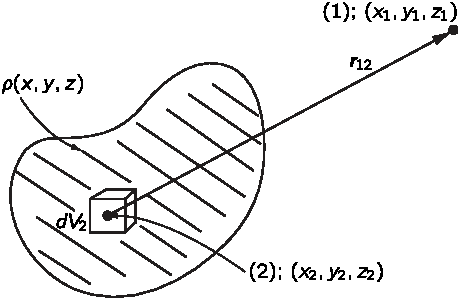
\includegraphics[width=0.6\linewidth]{fyz_fig0202.pdf}
      \caption{Elektrické pole \(\vec{E}\) v bodě \(1\) nějakého rozdělení nábojů získáme 
               integrálem přes toto rozdělení. Bod \(1\) se může nacházet i uvnitř rozdělení}
      \label{fyz:fig0202}
    \end{figure}
    Při používání Coulombova zákona při takovém přístupu nahradíme sumu ve vztahu  
    (\ref{fyz:eq276}) integrálem přes objem obsahující náboje. Pak bude platit
    \begin{equation}\label{fyz:eq282}
      \vec{E}(1) = \bigints\limits_{\substack{\text{celý}\\\text{prostor}}}
                       \frac{1}{4\pi\varepsilon_0}
                       \frac{\varrho(2)\vec{e}_{12}}{r^2_{12}}\dd{V_2}
    \end{equation}
    Někteří lidé píšou raději
    \begin{equation*}
      \vec{e}_{12} = \frac{\vec{r}_{12}}{r_{12}}
    \end{equation*}
    kde \(\vec{r}_{12}\) je vektor posunutí z \(2\) do \(1\) (obr. \ref{fyz:fig0044}). 
    Integrál udávající \(\vec{E}\) je pak zapsán takto
    \begin{equation}\label{fyz:eq283}
      \vec{E}(1) = \bigints\limits_{\substack{\text{celý}\\\text{prostor}}}
                       \frac{1}{4\pi\varepsilon_0}
                       \frac{\varrho(2)\vec{r}_{12}}{r^3_{12}}\dd{V_2}
    \end{equation}
    Chceme-li pomocí těchto integrálů něco vypočítat, musíme je obvykle podrobně rozepsat. Pro 
    \(x\)-ovou složku rovností (\ref{fyz:eq282}) nebo (\ref{fyz:eq283}) bychom 
    pak psali rovnici \ref{fyz:eq284}.
            
    Tento vzorec nebudeme používat často. Napsali jsme jej sem pouze proto, abychom zdůraznili 
    fakt, že jsme úplně vyřešili všechny ty elektrostatické úlohy, ve kterých známe polohy všech 
    nábojů. Jsou dány náboje. Jaká jsou pole? Odpověď: vypočtěte tento integrál. Nic víc k tomu 
    není potřeba; pouze výpočet složitých trojrozměrných integrálů - přesně vzato, je to práce pro 
    počítač.

    Pomocí našich integrálů můžeme najít pole vytvářená nabitým rovinným nebo lineárním útvarem, 
    nabitou kulovou plochou anebo jiným udaným rozdělením náboje. Je důležité uvědomit si, že i 
    když budeme kreslit siločáry, hovořit o potenciálech nebo počítat divergence, výsledek už máme. 
    Závisí pouze na tvaru tohoto integrálu. Někdy je snadnější jej vypočítat nějakým důvtipným 
    trikem než jeho skutečným výpočtem. Ovládat takovéto postupy však vyžaduje naučit se mnohé 
    neobyčejné věci. V praxi je možná jednodušší nesnažit se dělat chytrého, a namísto toho 
    vypočítat vždy integrál přímo. I přesto se však nyní pokusíme být v této záležitosti důvtipnými 
    a budeme pokračovat analýzou některých jiných vlastností elektrického pole.
    
    \begin{gather}\label{fyz:eq284}
      E_x(x_1, y_1, z_1) = 
        \frac{1}{4\pi\varepsilon_0}
        \bigints\limits_{\substack{\text{celý}\\\text{prostor}}}\varrho(x_2, y_2, z_2)
        \frac{x_1-x_2}{[(x_1-x_2)^2+(y_1-y_2)^2+(z_1-z_2)^2]^{\frac{3}{2}}}\dd{x_2}\dd{y_2}\dd{z_2} 
    \end{gather} 

  %----------------------- Elektrický potenciál ----------------------------------------------------
  \section{Elektrický potenciál}\label{fyz:IIchapIVsecIII}
    \cite[s.~66]{Feynman02} Nejdříve probereme pojem elektrického potenciálu, který souvisí s prací 
    vykonanou při přenášení náboje z jednoho bodu do druhého. Mějme nějaké rozdělení náboje, které 
    vytváří elektrické pole. Ptejme se, kolik práce je třeba vynaložit na přenos malého náboje z 
    jednoho místa na druhé. Práce, která se vykonává přenášením náboje po nějaké dráze proti 
    elektrickým silám, je rovna záporně vzatému integrálu po této dráte ze složky elektrické síly 
    ve směru pohybu. 
     
    Přenášíme-li náboj z bodu \(a\) do bodu \(b\), bude platit
    \begin{equation*}
      W = -\int_{a}^{b}\vec{F}\dd{\vec{s}},
    \end{equation*}
    kde \(\vec{F}\) je elektrická síla působící na náboj v každém bodě a \(\dd{\vec{s}}\) je 
    diferenciální vektor posunutí podél dráhy (obr. \ref{fyz:fig0044}).

    \begin{figure}[ht!]  %\ref{fyz:fig0044}
      \centering
      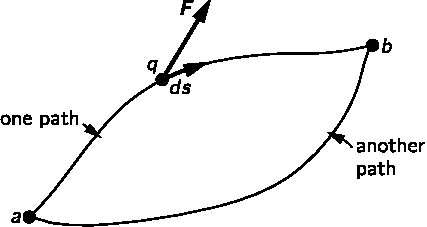
\includegraphics[width=0.6\linewidth]{fyz_fig0044.pdf}
      \caption{Práce konaná při přenesení náboje z \(a\) do \(b\) je rovna záporně vzatému 
        integrálu ze skalárního součinu \(\vec{F}\cdot d\vec{s}\) po dráze z \(a\) do \(b\)}
      \label{fyz:fig0044}
    \end{figure}    
    Pro naše účely je zajímavější uvažovat práci, která by se konala při přenášení jedné jednotky 
    náboje. Tehdy síla působící na náboj je číselně rovna intenzitě elektrického pole. Označíme-li 
    práci vykonanou proti elektrickým silám v tomto případě \(W_{jedn}\) můžeme psát
    \begin{equation}\label{fyz:eq285}
      W_{jedn} = -\int_{a}^{b}\vec{E}\dd{\vec{s}}.
    \end{equation}
    
    To, co dostaneme pomocí takového integrálu, obecně závisí na dráze, po které integrujeme. 
    Jestliže by integrál (\ref{fyz:eq285}) závisel na dráze od \(a\) do \(b\), mohli 
    bychom z pole získávat práci přenášením náboje do \(b\) po jedné dráze a pak zpět do \(a\) po 
    jiné. Do \(b\) bychom šli po dráze, pro kterou je \(W\) menší, a \emph{zpět} po jiné dráze, 
    odčerpávající \emph{víc} práce, \emph{než} vkládáme.
    
    Získávat energii z pole - na tom není v principu nic nemožného. Opravdu se setkáme s poli, kde 
    to možné je. Může se stát, že když pohybujete nábojem, působíte silami na jinou část 
    „mechanizmu“. Pohybuje-li se mechanizmus proti síle, ztrácí energii, přičemž celková energie v 
    přírodě se nemění. Avšak v elektrostatice takový „mechanizmus“ není. Víme, jaké síly působí 
    zpětně na zdroje pole. Jsou to coulombovské síly působící na náboje, které jsou původci pole. 
    Mají-li Ostatní náboje v prostoru pevné polohy, což předpokládáme pouze v elektrostatice, 
    nevykonávají tyto zpětné síly při působení práci. Neexistuje žádný způsob, jak z nich získat 
    energii, samozřejmě za předpokladu, že v elektrostatických situacích platí princip zachování 
    energie. Věříme, že platí, ale teď ukážeme, že to musí vyplývat z Coulombova zákona pro 
    sílu.         
    
    Uvažujme nejdříve, co se stane v poli vyvolaném jediným nábojem \(q\), Nechť je bod \(a\) ve 
    vzdálenosti \(r_1\) od \(q\) a bod \(b\) ve vzdálenosti \(r_2\). Nyní z \(a\) do \(b\) přenesme 
    jiný náboj, který budeme nazývat „zkušebním“ nábojem a jehož velikost zvolíme rovnou jedné 
    jednotce. Začněme s tou dráhou, která je ze všech možných drah pro výpočet nejjednodušší. Náš 
    zkušební náboj přeneseme nejdřív po oblouku kružnice a pak podél poloměru, jak to znázorňuje 
    obr. \ref{fyz:fig0203a}. Najít práci vykonanou na této speciální dráze je dětskou hrou 
    (jinak bychom ji nebyli zvolili). Především vůbec žádná práce se nevykoná na dráze z \(a\) do 
    \(a'\). Pole je radiální (podle Coulombova zákona), takže jeho intenzita je kolmá na směr 
    pohybu. Dále na dráze z \(a'\) do \(b\) má intenzita pole směr pohybu a mění se jako 
    \(\frac{1}{r^2}\). Práce vykonaná přenosem zkušebního náboje z \(a\) do \(b\) bude
    \begin{equation}\label{fyz:eq286}
     -\int_{a}^{b}\vec{E}\dd{\vec{s}} = 
       -\frac{q}{4\pi\varepsilon_0}\int_{a'}^{b}\frac{\dd{r}}{r^2} = 
       -\frac{q}{4\pi\varepsilon_0}\left(\frac{1}{r_{a}}-\frac{1}{r_{b}}\right).  
    \end{equation}
    \begin{figure}[ht!]
      \centering
      \subcaptionbox{\label{fyz:fig0203a}}{\luafigure[0.45]{fyz_fig0203a.pdf}}
      \subcaptionbox{\label{fyz:fig0203b}}{\luafigure[0.45]{fyz_fig0203b.pdf}}  
      \caption{Přenášením zkušebního náboje z a do b po obou těchto drahách se koná stejná práce}
      \label{fyz:fig0203}
    \end{figure}
    
    Vezměme nyní jinou jednoduchou dráhu, např. takovou, jaká je znázorněná na obr. 
    \ref{fyz:fig0203b}. Chvíli vede po oblouku kružnice, potom chvíli radiálně, potom  opět 
    po oblouku a potom radiálně atd. Předně, když jdeme po oblouku kružnice, práci nevykonáváme. 
    Když jdeme po radiálním úseku, musíme integrovat \(\frac{1}{r^2}\). Na prvním radiálním úseku 
    integrujeme z \(r_{a}\) do \(r_{a'}\), na druhém úseku z \(r_{a'}\) do \(r_{a''}\) atd. Součet 
    všech těchto integrálů dá totéž jako jediný integrál přímo z \(r_{a}\) do \(r_{b}\). Pro tuto 
    dráhu dostáváme stejný výsledek, jaký jsme dostali v případě první dráhy. Je zřejmé, že tentýž 
    výsledek bychom dostali pro jakoukoliv dráhu, která se skládá z libovolného počtu takovýchto 
    úseků.
    
    Jak to bude v případě hladkých drah? Dostali bychom tentýž výsledek? O této otázce jsme 
    hovořili už ve 13. kapitole 1. dílu. Na základě stejných důvodů, které jsme použili tam, můžeme 
    udělat závěr, že práce vykonaná při přenášení jednotkového náboje z \(a\) do \(b\) nezávisí na 
    dráze.   
    \begin{equation*}
      W_{\substack{\text{jedn}\\ a-b}} = 
       - \int\limits_{\substack{a\\\text{jakákoliv}\\\text{dráha}}}^b\vec{E}\dd{\vec{s}}.
    \end{equation*}      

    \begin{figure}[ht!]  %\ref{fyz:fig0045}
      \centering
      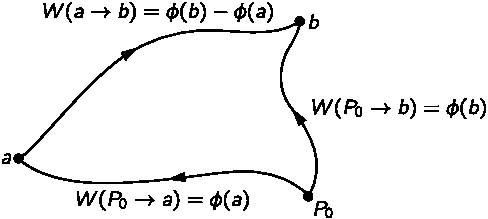
\includegraphics[width=0.6\linewidth]{fyz_fig0045.pdf}
      \caption{Práce vykonaná při postupu po jakékoliv dráze z \(a\) do \(b\) je rovna záporně     
        vzaté práci z nějakého bodu \(P_0\) do \(a\) zvětšené o práci z \(P_0\) do \(b\)}
      \label{fyz:fig0045}
    \end{figure}
    Protože vykonaná práce závisí pouze na koncových bodech, je možné ji udat jako rozdíl dvou 
    čísel. Přesvědčíme se o tom následujícím způsobem. Zvolme vztažný bod \(P_0\) a domluvme se, že 
    budeme počítat náš integrál použitím dráhy, která bude vždy procházet bodem \(P_0\). Nechť 
    \(\varphi(a)\) označuje práci vykonanou proti poli při přechodu z \(P_0\) do bodu \(a\) a 
    \(\varphi(b)\) práci vykonanou při přechodu z \(P_0\) do bodu \(b\) (obr. 
    \ref{fyz:fig0045}). Práce vykonaná při přechodu z \(a\) do \(P_0\) (cestou do \(b\)) 
    je záporně vzaté \(\varphi(a)\), takže bude platit

    \begin{equation}\label{fyz:fey_eq_elstat21}
     - \int\limits_{a}^{b}\vec{E}\dd{\vec{s}} = \varphi(b) - \varphi(a). 
    \end{equation}
    Protože tu bude vždy vystupovat pouze rozdíl hodnot funkce \(\varphi\) ve dvou bodech, ve 
    skutečnosti nepotřebujeme ani specifikovat polohu bodu \(P_0\). Jakmile jsme však zvolili 
    nějaký referenční bod, hodnota \(\varphi\) je už určena pro každý bod v prostoru; \(\varphi\) 
    je tedy \emph{skalární pole}. Je funkcí \(x, y, z\). Tuto skalární funkci nazýváme 
    \emph{elektrostatickým potenciálem} v libovolném bodě.

    \emph{Elektrostatický potenciál:}
     \begin{equation}\label{fyz:fey_eq_elstat22}
       \varphi(P) = - \int\limits_{P_0}^{P}\vec{E}\dd{\vec{s}} = \varphi(b) - \varphi(a). 
     \end{equation} 
    
    Často je pohodlné volit vztažný	bod v nekonečnu. V případě jednotlivého	náboje nacházejícího se 
    v počátku souřadnicové soustavy pak s ohledem	na vztah (\ref{fyz:eq286}) pro 
    potenciál 
    \(\varphi\) v nějakém bodě \((x, y, z)\) dostaneme
    \begin{equation}\label{fyz:fey_eq_elstat23}
     \varphi(x, y, z) = \frac{q}{4\pi\epsilon_0}\frac{1}{r}. 
    \end{equation}

    Elektrické pole několika nábojů je možné napsat jako součet elektrického pole prvního, druhého, 
    třetího atd. náboje. Integrujeme-li součet, abychom našli potenciál, dostaneme součet 
    integrálů. Každý z těchto integrálů představuje potenciál jednoho z nábojů. Usuzujeme tak 
    proto, že potenciál množiny nábojů je součtem potenciálů jednotlivých nábojů. Princip 
    superpozice platí tedy i pro potenciály. Stejnými úvahami, kterými jsme našli elektrické pole 
    skupiny nábojů a rozdělení nábojů, můžeme dostat úplné vzorce i pro potenciál \(\varphi\) v 
    nějakém bodě, který označíme \(1\):
    \begin{align}
     \varphi(1) &= 
       \sum\limits_{j}\frac{q_j}{4\pi\epsilon_0}\frac{1}{r_{1j}}     \label{fyz:fey_eq_elstat24} \\ 
     \varphi(1) &= 
       \frac{1}{4\pi\epsilon_0}\int\frac{\varrho(2)}{r_{12}}\dd{V_2} \label{fyz:fey_eq_elstat25}
    \end{align}
     	    
    Zapamatujte si, že potenciál \(\varphi\) má fyzikální význam: je to potenciální energie, kterou 
    by měl jednotkový náboj, přenesl-li by se z nějakého vztažného bodu do daného bodu v prostoru.
    
  %----------------------- Gradient potenciálu ´----------------------------------------------------
  \section{\texorpdfstring{\(\vec{E} = -\nabla\varphi\)}{Gradient potenciálu}}\label{fyz:IIchapIVsecIV}
    \cite[s.~70]{Feynman02} Kdo potřebuje potenciál \(\varphi\). Vždyť síly působící na náboje jsou 
    určené hodnotami \(\vec{E}\) -\emph{elektrickým polem}. Vtip je v tom, že \(\vec{E}\) je možné 
    snadno dostat z \(\varphi\) výpočtem derivace. Uvažujme dva body, jeden v \(x\) a druhý v \((x 
    + dx)\), ale u obou při stejných \(y\) a \(z\), a ptejme se, jak velká práce se vykoná při 
    přenášení jednotkového náboje z jednoho bodu do druhého. Jde o dráhu podél 	horizontály z \(x\) 
    do \(x + dx\) Vykonaná práce je dána rozdílem potenciálů v obou bodech:
    \begin{equation*}
     \Delta W = \varphi(x+dx, y, z) - \varphi(x, y, z) = \pder{\varphi}{x}\Delta x.
    \end{equation*}
    Ale práce vykonaná po téže dráze proti poli je
    \begin{equation*}
     \Delta W = - \int\vec{E}\cdot\dd{\vec{s}} = - E_x \Delta x.
    \end{equation*}
    Vidíme že,
    \begin{equation}\label{fyz:fey_eq_elstat26}
    E_x = -\pder{\varphi}{x}
    \end{equation}
    Podobně \(E_y = -\pder{\varphi}{y}\), \(E_z = -\pder{\varphi}{z}\) - nebo, napsané souborné 
    symbolikou vektorové analýzy,
    \begin{equation}\label{fyz:fey_eq_elstat27}
    \vec{E} = -\nabla\varphi.
    \end{equation}    
    Tato rovnice představuje diferenciální tvar vztahu (\ref{fyz:fey_eq_elstat22}). Jakoukoliv 
    úlohu, v níž jsou dány náboje, je možné řešit výpočtem potenciálu pomocí 
    (\ref{fyz:fey_eq_elstat24}) nebo (\ref{fyz:fey_eq_elstat25}) a použitím vztahu 
    (\ref{fyz:fey_eq_elstat27}) pro výpočet pole. Vztah (\ref{fyz:fey_eq_elstat27}) souhlasí i s 
    tím, co jsme zjistili o vektorovém počtu: pro každé skalární pole platí
    \begin{equation}\label{fyz:fey_eq_elstat28}
     \int\limits_{a}^{b}\ngrad{\varphi}\cdot\dd{\vec{s}} = \varphi(b) - \varphi(a)
    \end{equation}     
    
    Podle vztahu (\ref{fyz:fey_eq_elstat25}) je skalární potenciál \(\varphi\) dán trojrozměrným 
    integrálem podobným tomu, který jsme měli pro \(\vec{E}\). Je proto vůbec výhodné počítat 
    \(\varphi\) místo \(\vec{E}\)? Ano. Pro \(\varphi\) máme jen jeden integrál, zatímco pro 
    \(\vec{E}\) jsou zapotřebí tři integrály, neboť jde o vektor. Kromě toho \(\frac{1}{r}\) je 
    obvykle jednodušší integrovat než \(\frac{x}{r^3}\). V mnoha praktických případech se ukazuje, 
    že je poněkud jednodušší vypočítat \(\varphi\) a pak najít elektrické pole pomocí gradientu, 
    než počítat tři integrály pro \(\vec{E}\). Je to čistě praktická záležitost
    
    Potenciál \(\varphi\) má kromě toho i hlubší fyzikální význam. Ukázali jsme, že \(\vec{E}\) v 
    Coulombově zákoně je odvozeno z \(\vec{E}= -\grad{\varphi}\), kdy \(\varphi\) je dáno vztahem 
    (\ref{fyz:fey_eq_elstat22}). Ale z vektorového počtu víme, že \textbf{je-li \(\vec{E}\) rovno 
    gradientu skalárního pole, pak \(\rot{E}\) musí být rovna nule}:
    \begin{equation}\label{fyz:fey_eq_elstat29}
     \nrot{E} = 0 
    \end{equation}
    
    Toto je však právě naše druhá základní rovnice elektrostatiky (\ref{fyz:eq278b}). 
    Ukázali jsme tak, že Coulombův zákon definuje pole \(\vec{E}\), které splňuje tuto podmínku. 
    Dosud je vše v pořádku.
    
    Ve skutečnosti jsme dokázali, že \(\nrot{E}\) je rovno nule, dřív než jsme definovali 
    potenciál. Ukázali jsme, že práce vykonaná na uzavřené dráze je rovna nule, tj. že
    \begin{equation*}
     \oint\vec{E}\cdot\dd{\vec{s}} = 0 
    \end{equation*}  
    pro \emph{každou dráhu}. V kapitole \ref{fyz:IIchapIII} jsme se přesvědčili, že pro 
    každé takové pole musí být \(\nrot{E}\) všude rovno nule. Elektrické pole v elektrostatice je 
    tedy příkladem pole s \emph{nulovou rotací}. 
    
    Můžeme se pocvičit ve vektorovém počtu tím, že dokážeme tvrzení, že \(\nrot{E}=0\), a to 
    výpočtem složek vektoru \(\nrot{E}\) pro pole bodového náboje dané vztahem 
    (\ref{fyz:eq280}). Bude-li výsledkem výpočtu nula, pak podle principu superpozice 
    bychom dostali nulu pro jakékoliv rozdělení náboje.
    
    Je třeba poukázat na důležitou skutečnost. Pro libovolnou radiální sílu nezávisí vykonaná práce 
    na dráze a existuje potenciál. Přemýšlíte-li o tom, přesvědčíte se, že všechny úvahy, které 
    jsme provedli výše, abychom ukázali, že integrál práce nezávisí na dráze, byly postaveny pouze 
    na faktu, že síla jednotlivého náboje je radiální a kulově symetrická. Při těchto úvahách jsme 
    nevyužívali skutečnost, že závislost síly na vzdálenosti je dána vztahem \(\frac{1}{r^2}\), 
    mohlo by tedy jít o libovolnou závislost na \(r\). Existence potenciálu a skutečnost, že 
    \(\nrot{E}\) je rovna nule, pramení opravdu jen ze symetrie a směru elektrostatických sil. 
    Proto vztahy (\ref{fyz:fey_eq_elstat28}) nebo (\ref{fyz:fey_eq_elstat29}), mohou obsahovat 
    pouze část zákonů elektřiny. 
 
  %------------------------ Gradient potenciálu ´---------------------------------------------------
  \section{Tok pole \texorpdfstring{\(\vec{E}\)}{E}}\label{fyz:IIchapIVsecV}
    \cite[s.~72]{Feynman02} Nyní odvodíme rovnici pole, která závisí právě a přímo na skutečnosti, 
    že ve jmenovateli zákona síly vystupuje druhá mocnina vzdálenosti. To, že se pole mění nepřímo 
    úměrně s druhou mocninou vzdálenosti, se někomu zdá být „jedině přirozeným“, neboť „je to 
    způsob, kterým se šíří všechno“. Vezměme si světelný zdroj, z něhož vychází světlo: množství 
    světla procházející základnou kužele s vrcholem ve zdroji je stejné bez ohledu na to, jak 
    daleko je základna od zdroje. Tak to musí být, má-li se světelná energie zachovávat. Množství 
    světla připadající na jednotku plochy, tedy intenzita osvětlení, se musí měnit přímo úměrně 
    plošnému obsahu základny kužele, tj. nepřímo úměrně druhé mocnině vzdálenosti od zdroje. Ze 
    stejného důvodu by se zajisté mělo měnit i elektrické pole. Ale nic takového jako „stejný“ 
    důvod neexistuje. Nikdo nemůže říci, že elektrické pole je mírou toku něčeho podobného jako 
    světlo, které se musí zachovávat. Kdybychom měli takový „model“ elektrického pole, v němž by 
    vektor pole udával směr a rychlost, tj. představoval by tok nějakých drobných vyletujících 
    „kulek“, a kdyby náš model vyžadoval, aby se tyto kulky zachovávaly a žádná by nemohla zmizet, 
    pokud už byla vystřelena, tak bychom řekli, že můžeme nevyhnutelnost zákona nepřímé úměrnosti 
    druhé mocnině vzdálenosti „pochopit“. Na druhé straně nevyhnutelně musí existovat nějaký 
    matematický způsob, jak tuto fyzikální představu vyjádřit. Kdyby elektrické pole bylo něčím 
    takovým jako zachovávající se vyletující kulky, měnilo by se nepřímo úměrně s druhou mocninou 
    vzdálenosti, a takové chování bychom byli schopni popsat rovnicí - což je čistě matematická 
    záležitost. Není tedy nic špatného na tom, když se této představy podržíme, pokud ovšem 
    nebudeme tvrdit, že elektrické pole se opravdu skládá z kulek, ale budeme si vědomi toho, že 
    používáme model, který nám pomáhá najít správné matematické vyjádření.

    Předpokládejme, že jsme si na chvíli představili elektrické pole jako proud něčeho, co se 
    zachovává - všude, tj. mimo místa, kde se nacházejí náboje. (Proudění musí někde začínat.) 
    Představujeme si, že něco, ať už je to cokoliv, vytéká z náboje do okolního prostoru. Byl-li by 
    \(\vec{E}\) vektor takového toku (jako je \(\vec{h}\) v případě tepelného toku), v blízkosti 
    bodového zdroje by se vyznačoval závislostí \(\dfrac{1}{r^2}\). Tento model chceme nyní použít 
    k tomu, abychom našli způsob, jak dojít k zákonu nepřímé úměrnosti na druhé mocnině vzdálenosti 
    principiálnější nebo abstraktnější cestou místo toho, aby se prostě konstatovalo: „nepřímo 
    úměrné druhé mocnině“. (Snad se divíte, proč se chceme vyhnout přímému zformulování takového 
    jednoduchého zákona, a místo toho chceme dosáhnout téhož jinou cestou. Ale mějte trpělivost! 
    Ukáže se, že je to užitečné.)
    
    Ptáme se: Jaký je tok pole \(\vec{E}\) ven z libovolné uzavřené plochy v okolí bodového náboje? 
    Nejdříve vezměme jednoduchou plochu, jakou ukazuje obr. \ref{fyz:fig0204}. 
    
    \begin{figure}[ht!]  % \ref{fyz:fig0204}
      \centering
      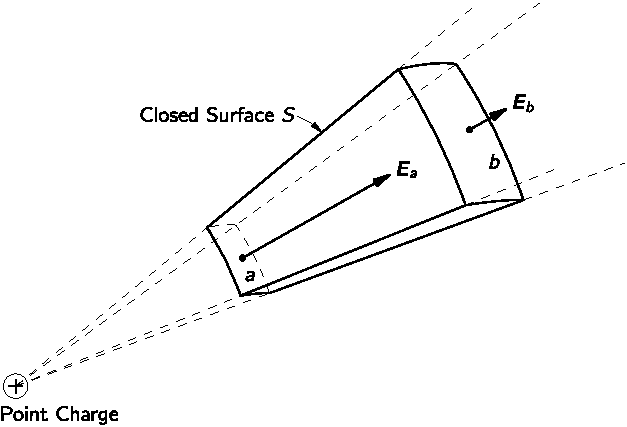
\includegraphics[width=0.7\linewidth]{fyz_fig0204.pdf}
      \caption{Tok vektoru \(\vec{E}\) z plochy \(S\) je roven nule}
     \label{fyz:fig0204} 
    \end{figure}
    
    Má-li pole \(\vec{E}\) charakter toku, musí být celkový tok z takové krabičky roven nule. Tento 
    výsledek opravdu dostaneme, rozumíme-li „tokem“ z této plochy plošný integrál normálové složky 
    vektoru \(\vec{E}\), tj. veličinu, kterou jsme nazvali tokem pole \(\vec{E}\). V případě 
    radiálních (rovnoběžných se spojnicí k náboji) stěn je normálová složka \(\vec{E}\) nulová. V 
    případě kulových čelních stěn je normálová složka \(E_n\) rovna velikosti vektoru \(\vec{E}\) - 
    se záporným znaménkem u menší a s kladným u větší stěny. Velikost vektoru \(\vec{E}\) klesá 
    jako \(\dfrac{1}{r^2}\), ale plošný obsah stěny je přímo úměrný veličině \(r\), takže jejich 
    součin na \(r\) nezávisí. Tok vektoru \(\vec{E}\) do stěny \(a\) se právě ruší tokem ze stěny 
    \(b\). Celkový tok z \(S\) je roven nule, což je rovnocenné s tvrzením, že pro tuto plochu je
    \begin{equation}\label{fyz:fey_eq_elstat30}
    \oint_SE_n\dd{S} = 0.
    \end{equation}
    
    \begin{figure}[ht!]
      \centering
      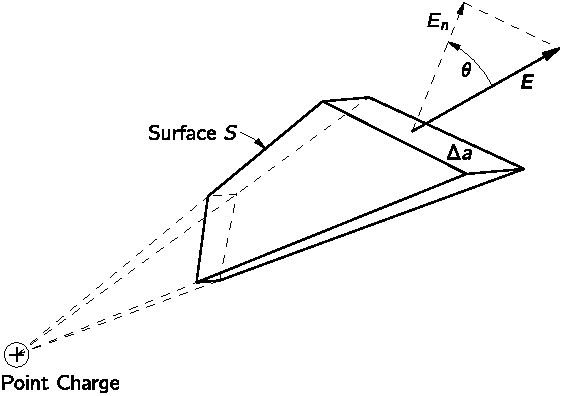
\includegraphics[width=0.7\linewidth]{fyz_fig0205.pdf}
      \caption{Tok vektoru \(\vec{E}\) z plochy \(S\) je roven nule}
      \label{fyz:fig0205} 
    \end{figure}

    Dále ukážeme, že obě koncové plochy mohou být skloněny vzhledem k radiální přímce a integrál 
    (\ref{fyz:fey_eq_elstat30}) se přitom nezmění. Ačkoli to platí obecně, pro naše účely postačí 
    ukázat, že to platí, jsou-li koncové plochy malé, takže se ze zdroje jeví pod malým úhlem, 
    přesněji pod infinitezimálním úhlem. Na obr. \ref{fyz:fig0205} vidíme plochu \(S\) s 
    radiálními „stěnami“ a šikmými „konci“. Na obrázku nejsou koncové plochy malé, ale máte si 
    představit podobnou situaci s velmi malými koncovými plochami. Pak bude pole \(\vec{E}\) na 
    každé ploše dostatečně homogenní, abychom mohli pracovat pouze s jeho hodnotou ve středu 
    plochy. Skloníme-li plošku o úhel \(\vartheta\), její plošný obsah se zvětší 
    \(\dfrac{l}{cos\vartheta}\)krát. Ale \(E_n\) složka vektoru \(\vec{E}\) normálová k plošce, se 
    změní úměrně \(\cos\vartheta\). Součin \(E_n\cdot\Delta S\) se tedy nezmění. Tok z celé plochy 
    \(S\) zůstává nulový.
      
    \begin{figure}[ht!]
      \centering
      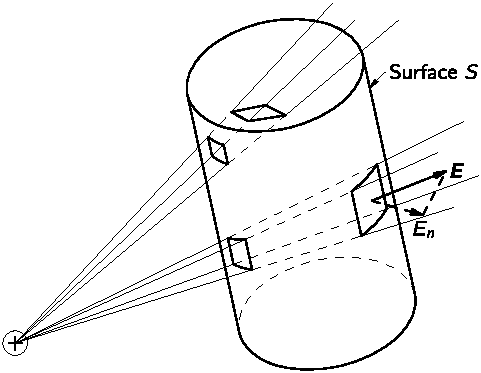
\includegraphics[width=0.7\linewidth]{fyz_fig0206.pdf}
      \caption{Každý objem lze považovat za úplně složený z infinitezimálních komolých kuželů. Tok 
               \(\vec{E}\) z jednoho konce kuželového segmentu se rovná zápornému toku z druhého 
               konce. Celkový tok z plochy \(S\) je proto roven nule.}
      \label{fyz:fig0206} 
    \end{figure}

    Nyní se snadno přesvědčíme, že tok z objemu vymezeného jakoukoliv plochou \(S\) musí být roven 
    nule. Každý objem je totiž možné si představit, jako kdyby se skládal z částí, podobných útvaru 
    znázorněnému na obr. \ref{fyz:fig0205}. Celá plocha \(S\) se přitom rozdělí do párů 
    koncových plošek, a protože vtoky a výtoky z těchto koncových plošek se v jednotlivých párech 
    navzájem ruší, celkový tok z plochy \(S\) bude roven nule. Tuto představu ilustruje obr. 
    \ref{fyz:fig0206}. Dostáváme úplně obecný výsledek, že celkový tok pole \(\vec{E}\) ven 
    z jakékoliv plochy \(S\) v poli bodového náboje je roven nule. 

    \begin{figure}[ht!]
      \centering                  
      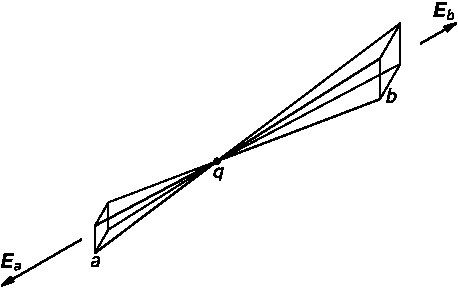
\includegraphics[width=0.6\linewidth]{fyz_fig0207.pdf}
      \caption{Nachází-li se náboj uvnitř plochy, tok z ní není roven nule.}
      \label{fyz:fig0207}  
    \end{figure} 
                  
    Ale pozor! Náš důkaz platí pouze tehdy, neobklopuje-li plocha \(S\) náboj. Co by se stalo, 
    kdyby se bodový náboj nacházel uvnitř plochy? Opět můžeme naši plochu rozdělit na páry plošek, 
    které jsou vymezeny radiálními přímkami procházejícími nábojem tak, jak to ukazuje obr. 
    \ref{fyz:fig0207}. Opět jsou tu toky  oběma ploškami stejně velké, z týchž důvodů jako dříve, 
    pouze teď mají stejné znaménko. Tok z plochy, která obklopuje náboj, není nulový. Jaký tedy je? 
    Můžeme ho najít malým trikem. Předpokládejme, že náboj „odstraníme“ z „vnitřku“ tím, že ho 
    obalíme malou plochou S uloženou úplně uvnitř původní plochy \(S\) (obr. \ref{fyz:fig0208a})
   
    Pak se v objemu mezi oběma plochami \(S\) a \(S'\) žádný náboj nenachází. Celkový tok z tohoto 
    objemu (včetně toku plochou \(S'\)) je roven nule na základě úvah, jež jsme již uvedli. Z 
    těchto úvah vlastně vyplývá, že tok do objemu plochou \(S'\) je stejný jako tok z něj ven 
    plochou \(S\).

    \begin{figure}[ht!]
      \centering
      \subcaptionbox{\label{fyz:fig0208a}}{\luafigure[0.45]{fyz_fig0208a.jpg}}
      \subcaptionbox{\label{fyz:fig0208b}}{\luafigure[0.45]{fyz_fig0208b.jpg}}
      \caption{a) Nachází-li se náboj uvnitř plochy, tok z ní není roven nule; b) Tok kulovou 
              plochou obsahující uvnitř bodový náboj \(q\) je roven \(\dfrac{q}{\varepsilon}\)}
      \label{fyz:fig0208}
     \end{figure}
        
    Za \(S'\) můžeme zvolit plochu jakéhokoliv tvaru. Zvolme tedy kulovou plochu se středem v 
    náboji (obr. \ref{fyz:fig0208b}). Pak dokážeme snadno vypočítat tok touto plochou. 
        
    Je-li poloměr malé koule \(r\), má \(\vec{E}\) všude na jejím povrchu velikost
    \begin{equation*}
      \frac{1}{4\pi\varepsilon_0}\frac{q}{r^2}
    \end{equation*}
    a směr normály k povrchu. Celkový tok \(S'\) dostaneme, vynásobíme-li tuto normálovou složku 
    plošným obsahem plochy \(S'\):
    \begin{equation} \label{fyz:fey_eq_elstat31}
      \text{Tok plochou } S' = \left(\frac{1}{4\pi\varepsilon_0}\frac{q}{r^2}\right)(4\pi r^2)  
                             = \frac{q}{\varepsilon_0}
    \end{equation}
    je tedy roven hodnotě, která nezávisí na poloměru koule! Z toho vidíme, že tok ven z plochy 
    \(S\) je také roven \(\dfrac{q}{\varepsilon_0}\) - hodnotě, jež nezávisí na tvaru plochy \(S\), 
    pokud náboj \(q\) zůstává uvnitř.
    
    Naše výsledky můžeme napsat takto:
    \begin{equation}\label{fyz:fey_eq_elstat32}
      \limitint_{\mathclap{\substack{\text{jakákoliv}\\\text{uzavřená}\\\text{plocha }S}}} E_n\dd{S} = 
        \begin{dcases*}
           0                       & \(q\) vně \(S\) \\
           \frac{q}{\varepsilon_0} & \(q\) uvnitř \(S\)
        \end{dcases*}          
    \end{equation} 
        
    Vraťme se k naší analogii s kulkami a podívejme se, zda má smysl. Podle naší věty je celkový 
    tok kulek nějakou plochou roven nule, neobklopuje-li plocha zbraň vystřelující kulky. Je-li 
    zbraň obklopena plochou, ať má jakýkoliv tvar a velikost, počet kulek jí proletující je stejný 
    - určuje jej rychlost, jakou zbraň kulky vystřeluje. Pro zachovávající se kulky vypadá všechno 
    celkem rozumně. Ale poskytuje nám tento model něco víc, než dostáváme napsáním vztahu 
    (\ref{fyz:fey_eq_elstat32})? Nikomu se nepodařilo dosáhnout toho, aby tyto kulky dokázaly něco 
    víc, než zformulovat tento jediný zákon. Kromě toho už nevedou k ničemu, jen k omylům. Proto 
    dnes dáváme přednost čistě abstraktní představě elektromagnetického pole.

  %----------------------- Gaussův zákon. Divergence pole E ----------------------------------------
  \section{Gaussův zákon. Divergence pole \texorpdfstring{\(\vec{E}\)}{E}}\label{fyz:IIchapIVsecVI}
    \cite[s.~75]{Feynman02} Náš překrásný výsledek, tj. vztah (\ref{fyz:fey_eq_elstat32}), jsme 
    dokázali pro jediný bodový náboj. Nyní předpokládejme, že jsou dva náboje, náboj \(q_1\) v 
    jednom bodě a náboj \(q_2\) v jiném bodě. Tato úloha vypadá těžší. Elektrické pole, jehož 
    normálovou složku při toku integrujeme, je polem pocházejícím od obou nábojů, tj. 
    představuje-li \(\vec{E}_1\) elektrické pole, které by vytvořil samotný náboj \(q_1\) a 
    \(\vec{E}_2\) elektrické pole, které by vytvořil samotný náboj \(q_2\), celkové elektrické pole 
    \(\vec{E}=\vec{E}_1 + \vec{E}_2\). Tok každou uzavřenou plochou \(S\) je
    \begin{equation}\label{fyz:fey_eq_elstat33}
     \oint_S E_{1n} + E_{2n}\dd{S} = \oint_S E_{1n}\dd{S} + \oint_S E_{2n}\dd{S}.
    \end{equation}
    V případě obou nábojů je roven toku vyvolanému prvním nábojem plus tok vyvolaný druhým nábojem. 
    Jsou-li oba náboje na vnější straně \(S\), tok plochou \(S\) je nulový. Je-li \(q_1\), uvnitř 
    \(S\) a \(q_2\) mimo, první integrál dává \(\dfrac{q_1}{\varepsilon_0}\) a druhý nulu. 
    Obklopuje -li plocha oba náboje, bude každý dávat svůj příspěvek a dostáváme, že tok je 
    \(\dfrac{q_1+1_2}{\varepsilon_0}\). Obecné pravidlo je zřejmé: celkový tok z uzavřené plochy je 
    roven celkovému náboji uvnitř, dělenému \(\varepsilon_0\).
    
    Náš výsledek představuje důležitý obecný zákon elektrostatického pole, nazvaný \emph{Gaussův zákon}.
    \begin{align}
      \limitint_{\mathclap{\substack{\text{jakákoliv}      \\
                                     \text{uzavřená}       \\
                                     \text{plocha }S}}} E_n\dd{S} 
              &= \frac{\text{součet nábojů uvnitř}}{\varepsilon_0} \label{fyz:fey_eq_elstat34} \\
      \shortintertext{nebo}        
      \limitint_{\mathclap{\substack{\text{jakákoliv}       \\
                                            \text{uzavřená} \\
                                            \text{plocha }S}}} E_n\dd{S}
              &= \frac{Q_{\text{uvnitř}}}{\varepsilon_0}           \label{fyz:fey_eq_elstat35} \\
      \shortintertext{kde}
      Q_{\text{uvnitř}} 
              &= \sum\limits_{\text{uvnitř }S}q_i.                 \label{fyz:fey_eq_elstat36}  
    \end{align}
    Popíšeme-li rozmístění nábojů pomocí hustoty náboje \(\varrho\), můžeme to chápat tak, že každý 
    infinitezimální objem \(dV\) obsahuje „bodový“ náboj \(\varrho dV\). Součet všech nábojů pak 
    bude dán integrálem
    \begin{equation}\label{fyz:fey_eq_elstat37}
     Q_{\text{uvnitř}} = \limitint_{\mathclap{\substack{\text{objem}\\
                                                 \text{uvnitř }S}}} \varrho\dd{V}.
    \end{equation}
    
    Z našeho odvození vidíme, že Gaussův zákon vyplývá ze skutečnosti, že mocnitel v Coulombově 
    zákoně je roven přesně dvěma. Pole se zákonem \(\dfrac{1}{r^3}\) nebo jakékoliv pole se zákonem 
    \(\dfrac{1}{r^n}\), kde \(n\neq2\), by ke Gaussovu zákonu nevedlo. Gaussův zákon tedy není 
    právě ničím jiným než vyjádřením (v odlišném tvaru) Coulombova zákona síly, která působí mezi 
    dvěma náboji. Opravdu, zpětným postupem můžete z Gaussova zákona odvodit Coulombův zákon. Oba 
    tyto zákony jsou zcela ekvivalentní, máme-li na paměti, že síly působící mezi náboji jsou 
    radiální\footnote{A kulové symetrické neboli centrální}.
    
    Nyní bychom rádi napsali Gaussův zákon pomocí derivací. Abychom to udělali, použijeme Gaussův 
    zákon na povrch infinitezimální krychle. V kapitole \ref{fyz:IIchapIII} jsme ukázali, 
    že tok vektoru \(\vec{E}\) z takovéto krychle je roven hodnotě \(\nabla\cdot\vec{E}\) 
    vynásobené objemem krychle \(dV\)! Náboj uvnitř \(dV\) je podle definice roven \(\varrho dV\), 
    takže z Gaussova zákona dostaneme
    \begin{equation}\label{fyz:fey_eq_elstat38}
     \ndiver{E}\dd{V} = \frac{\varrho\dd{V}}{\varepsilon_0} \quad 
     \text{nebo} \quad
     \ndiver{E}       = \frac{\varrho}{\varepsilon_0}
    \end{equation}
    Diferenciální tvar Gaussova zákona představuje první z našich fundamentálních rovnic pole v 
    případě elektrostatiky (rovnice \ref{fyz:eq278a}). Ukázali jsme tím, že obě rovnice 
    elektrostatiky (rovnice \ref{fyz:eq278a} a \ref{fyz:eq278b}) jsou 
    ekvivalentní Coulombovu zákonu síly. Dále se budeme zabývat jedním příkladem použití Gaussova 
    zákona. (Později se dostaneme k mnohem většímu množství takových příkladů.)
    
  %----------------------- Pole nabité koule -------------------------------------------------------
  \section{Pole nabité koule}\label{fyz:IIchapIVsecVII}
    Jednou z těžkých úloh, s nimiž jsme se setkali, když jsme studovali teorii gravitace, bylo 
    dokázat, že síla pocházející z pevné koule je na jejím povrchu taková, jako kdyby všechna látka 
    byla soustředěna ve středu koule. Newton po mnoho let svou teorii gravitace nepublikoval, 
    protože si nebyl jistý, zda je toto tvrzení pravdivé. Dokázali jsme jej ve kapitole 
    \ref{fyz:IchapXIII} \ref{part:FYZI}. dílu tak, že jsme vypočítali integrál potenciálu a pak 
    jsme pomocí gradientu našli gravitační sílu. Nyní můžeme tuto větu dokázat jednodušším 
    způsobem. Tentokrát budeme dokazovat jí odpovídající větu pro homogenně elektricky nabitou 
    kouli. (Protože zákony elektrostatiky jsou stejné jako zákony gravitace, mohl by být tentýž 
    důkaz proveden i pro gravitační pole.) \cite[s.~77]{Feynman02}
    
    Ptáme se: Jaké je elektrické pole \(\vec{E}\) v bodě \(P\), který se nachází někde mimo kouli s 
    rovnoměrným rozdělením náboje? Protože tam není žádný význačný směr, můžeme předpokládat, že 
    \(\vec{E}\) směřuje od středu koule. Uvažujme myšlenou kulovou plochu, která je koncentrická s 
    nabitou koulí a prochází bodem \(P\) (obr. \ref{fyz:fig0209}). Tok směrem ven z 
    této plochy je

    \begin{equation*}
      \int E_n\dd{S} = E\cdot4\pi R^2.
    \end{equation*} 
    Podle Gaussovy věty je tento tok roven celkovému náboji koule \(Q\) (dělenému 
    \(\varepsilon_0\)):
    \begin{equation*}
      E\cdot4\pi R^2 = \frac{Q}{\varepsilon_0}.
    \end{equation*} 
    neboli
    \begin{equation*}
      E  = \frac{1}{4\pi\varepsilon_0}\frac{Q}{r^2},
    \end{equation*}
    \noindent což je stejný vzorec, jaký bychom měli pro bodový náboj \(Q\). Newtonovu úlohu jsme 
    dokázali snáze než pomocí integrálu. To je, pravda, jen zdánlivě jednodušší - nějaký čas vám 
    trvalo, než jste porozuměli Gaussovu zákonu, takže se můžete domnívat, že ve skutečnosti jste 
    ani žádný čas neušetřili. Když však budete používat tuto větu stále častěji, začne se to 
    splácet. Je to otázka efektivnosti.    
    \begin{figure}[ht!]
      \centering
      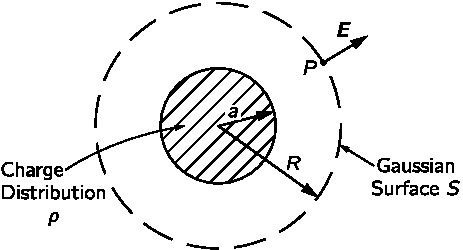
\includegraphics[width=0.7\linewidth]{fyz_fig0209.pdf}
      \caption{Použití Gaussova zákona na odvození pole homogenní nabité koule}
      \label{fyz:fig0209}  
    \end{figure}
   

  %----------------------- Siločáry, ekvipotenciální plochy ----------------------------------------
  \section{Siločáry, ekvipotenciální plochy}\label{fyz:IIchapIVsecVIII}
    Nyní bychom rádi uvedli geometrický popis elektrostatického pole. Oba zákony elektrostatiky - 
    první, že tok je přímo úměrný náboji uvnitř, a druhý, že elektrické pole je gradientem 
    potenciálu - je rovněž možno interpretovat geometricky. Ilustrujeme to těmito dvěma příklady. 
    Nejdříve mějme pole bodového náboje. Nakreslíme křivky ve směru pole, tj. křivky, jejichž tečny 
    mají všude směr vektoru pole (obr. \ref{fyz:fig0210}). Jsou to tzv. siločáry. 
    \cite[s.~78]{Feynman02}
    
    V každém bodě ukazují směr elektrického vektoru. Chceme však znázornit i jeho velikost. Můžeme 
    proto zavést pravidlo, že intenzitu elektrického pole bude reprezentovat „hustota“ siločar. 
    Hustotou siločar rozumíme počet siločar připadajících na jednotku plochy v rovině kolmé na 
    siločáry. Pomocí těchto pravidel můžeme vytvořit obraz elektrického pole. V případě bodového 
    náboje se musí hustota siločar zmenšovat podle zákona \(\frac{1}{r^2}\). Ale plošný obsah 
    kulové plochy kolmé na siločáry při každém poloměru \(r\) \emph{vzrůstá} s \(r^2\). 
    Zachováme-li tedy tentýž počet siločar ve \emph{všech} vzdálenostech od náboje, jejich hustota 
    zůstane přímo úměrná velikosti pole. Stejný počet siločar v každé vzdálenosti můžeme zabezpečit 
    tak, že budeme trvat na tom, aby siločáry byly \emph{souvislé}, tj. aby siločára, pokud už 
    jednou z náboje vyšla, nikde nekončila. Gaussův zákon vyjádřený jazykem siločar říká, že 
    siločáry mají začínat pouze v kladných nábojích a končit pouze v záporných nábojích. Počet 
    siločar \emph{vycházejících} z náboje \(q\) musí být roven \(\frac{q}{\varepsilon_0}\).
    
    Podobný geometrický obraz můžeme nyní najít i pro potenciál \(\varphi\). Nejjednodušší způsob 
    jak znázornit potenciál, je nakreslit plochy, na nichž je \(\varphi\) stálé. Říkáme jim 
    ekvipotenciální plochy (hladiny), tj. plochy se stejným potenciálem. Jaký je geometrický vztah 
    ekvipotenciálních ploch k siločárám? Elektrické pole je gradientem potenciálu. Gradient udává 
    směr nejrychlejší změny potenciálu, a proto je kolmý na ekvipotenciální plochu (v každém bodě). 
    Kdyby totiž \(\vec{E}\) nebylo kolmé na ekvipotenciální plochu, mělo by v ní nenulovou složku. 
    Pak by se potenciál na ploše měnil a nebyla by ekvipotenciální plochou. Ekvipotenciální plochy 
    tedy musí všude svírat se siločárami elektrického pole pravý úhel.    
    \begin{figure}[ht!]
      \centering
      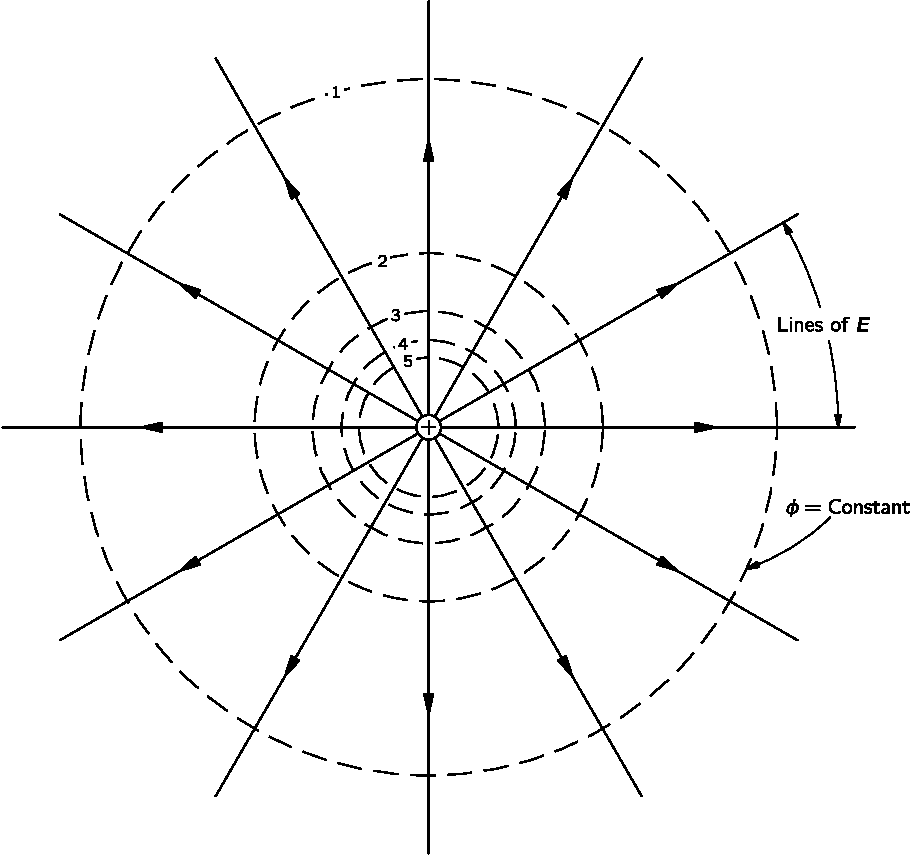
\includegraphics[width=0.8\linewidth]{fyz_fig0210.pdf}
      \caption{Siločáry a ekvipotenciální plochy v případě kladného bodového náboje.}
      \label{fyz:fig0210}
    \end{figure}
    
    V případě osamoceného bodového náboje jsou ekvipotenciálními plochami kulové plochy se středem 
    v náboji. Na obr. \ref{fyz:fig0210} jsme ukázali řez těmito kulovými plochami 
    procházejícími nábojem.
    
    Jako druhý příklad uvažujme pole v blízkosti dvou stejně velkých nábojů, jednoho kladného a 
    druhého záporného. Najít toto pole je snadné. Jde o superpozici polí pocházejících od každého z 
    těchto nábojů. Můžeme tedy dva obrázky, jako je obr. \ref{fyz:fig0210}, položit jeden 
    na druhý, ale to nejde. Dostali bychom tak siločáry, které se navzájem protínají, a to není 
    možné, neboť \(\vec{E}\) nemůže mít v jednom bodě dva různé směry. Nevýhoda popisu pole pomocí 
    siločar je nyní očividná. Geometrickými úvahami nelze snadno dospět k tomu, jaký průběh budou 
    mít nové siločáry. Ze dvou nezávislých obrazů siločar nemůžeme dostat jejich složený obraz. 
    Princip superpozice - jednoduchý a zároveň hluboký princip teorie elektrických polí - nemá v 
    popisu pole pomocí siločar jednoduchou reprezentaci.
    
    Představa siločar má však své použití, a proto bychom přece rádi nakreslili jejich obraz pro 
    dvojici nábojů stejné velikosti a opačných znamének.
    
    Vypočítáme-li pole ze vztahu (\ref{fyz:eq276}) a potenciály z 
    (\ref{fyz:fey_eq_elstat23}), můžeme siločáry a ekvipotenciální hladiny nakreslit. Výsledkem je 
    obr. \ref{fyz:eq276}. Tuto úlohu jsme však museli řešit nejdříve matematicky.
    \begin{figure}[ht!]
     \centering
     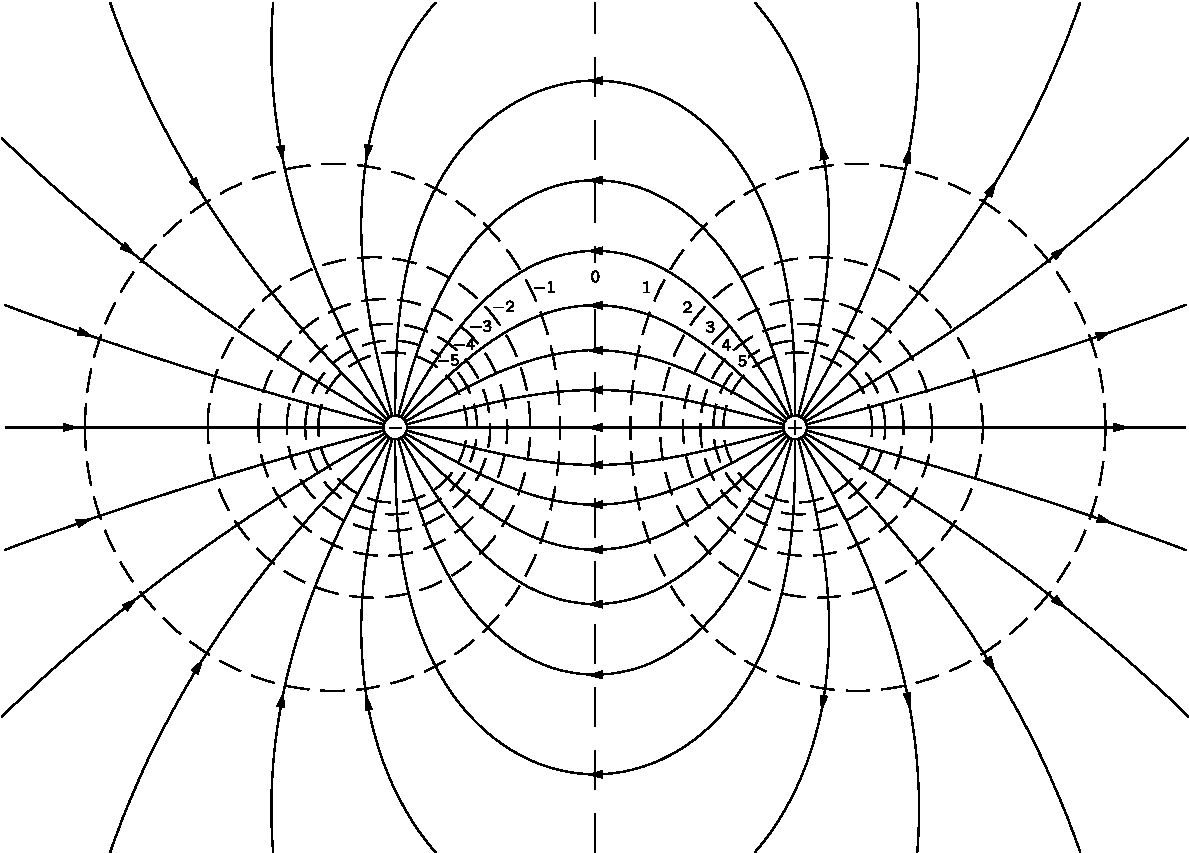
\includegraphics[width=\linewidth]{fyz_fig0211.pdf}
     \caption[Siločáry a ekvipotenciální plochy]{Siločáry a ekvipotenciální plochy v případě dvou 
              stejně velkých bodových nábojů s opačným znaménkem}
     \label{fyz:fig0211}
    \end{figure}


%} %tikzset
%~~~~~~~~~~~~~~~~~~~~~~~~~~~~~~~~~~~~~~~~~~~~~~~~~~~~~~~~~~~~~~~~~~~~~~~~~~~~~~~~~~~~~~~~~~~~~~~~~~